\section{The Encoder-Decoder architecture}\label{sec:encoder-decoder}

\subsection{From feature engineering to feature learning}

Machine learning algorithms take features as inputs and produce some output. How we represent features makes a huge difference on the performance of the learning algorithms.  Traditionally, approaches to machine learning require a strong \textbf{feature engineering} approach, meaning that the designer has to carefully choose features and their representation before feeding them into the algorithm. When facing complex problems like computer vision, this approach came up with sophisticated representations, such as HOG (Histogram of Oriented Gradients) for representing image features.

Due to such representations, there is a difference to be made between the \textit{raw inputs}, and the features which are input to the model. For example, in face recognition, the pixels of a picture are the raw input, while the HOG features of the image can be the actual input to the model.

Someone came up with the idea that we can use an algorithm to learn the feature representation itself, aptly called \textbf{feature learning}. Deep learning uses a neural network model to achieve this task. In point of fact, feature learning is accomplished by the first layers of a neural network, which map raw inputs to efficient feature representations. The last layers (typically fully connected layers) mix and match and combine these features to produce an output.

\subsection{The encoder-decoder architecture}

The \textbf{encoder-decoder architecture} explicitly aims to leverage this ability of neural networks to learn efficient representations. It is a neural network design pattern that consists of two main components, the \textit{encoder} and the \textit{decoder}.  The \textbf{encoder} maps raw inputs to feature representations, and these representations are then passed to the \textbf{decoder}, which has to produce an output. This is commonly referred to as the encoder-decoder framework, and its general architecture is shown in \cref{fig:encoder-decoder}

\begin{figure}[hpt]
	\centering
	\includesvg{images/ch3/encoder-decoder.svg}
	\caption{The encoder-decoder architecture.}
	\label{fig:encoder-decoder}
\end{figure}

Theoretically, encoder and decoder parts can be used independently of each other. For instance, an encoder RNN can be used to encode the features of an incoming email as a \textit{features vector}, which is then used as input to a Fully-Connected Layer (FCL) to predict whether the email is spam or not. However, neural encoder and decoders are often used in a tightly coupled manner, meaning that the system is trained as a whole. This approach, known as \textbf{end-to-end}, is been increasingly used due to a combination of good performance and less engineering effort.

The encoder-decoder architecture is enormously popular in the fields of computer vision and natural language processing, and may adopt very different forms. In some cases, the same type of network is used for both the encoder and the encoder.

For example, \cref{fig:cnn-cnn} depicts an example of a pure convolutional encoder-decoder architecture (there is no fully connected layer). This model is used to perform semantic segmentation of an image. The left half of the network (the encoder) maps raw image pixels to a rich representation consisting of feature vectors. The right half of the network (the decoder) takes these features and upsamples them to produce a sparse feature map which is fed to a soft-max for pixel-wise classification.

\begin{figure}[hpt]
	\centering
	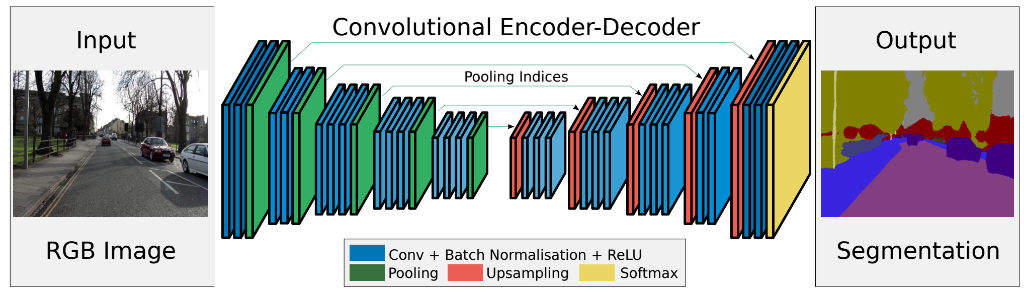
\includegraphics[scale=0.45]{images/ch3/cnn-cnn.png}
	\caption{Convolutional encoder-decoder for image segmentation in the SeqNet architecture \citep{Badrinarayanan2017}}
	\label{fig:cnn-cnn}
\end{figure}

Encoder-decoder networks based on RNN are very common in problems requiring \textit{sequence-to-sequence (seq2seq)} modelling, such as translation, summarising and question-answering. For example, \cref{fig:rnn-rnn} shows an example of a model used to generate automatic responses to incoming emails. The left half of the network encodes the email into a feature vector, and the right half of the network decodes the feature vector to produce word predictions. 

\begin{figure}[hpt]
	\centering
	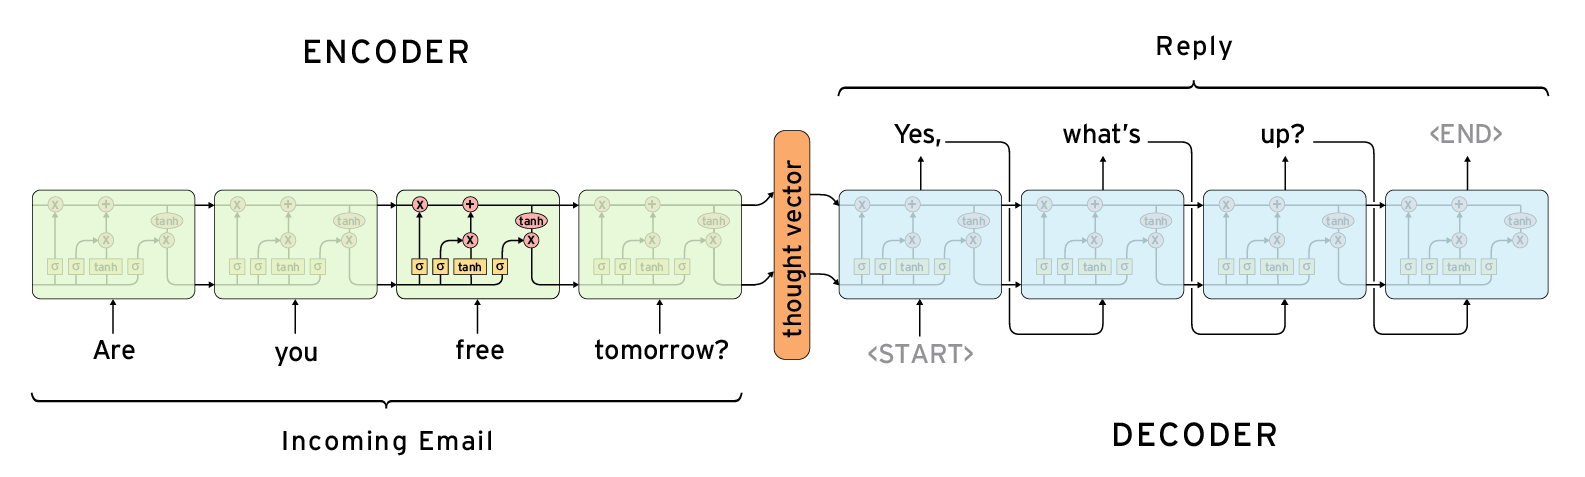
\includegraphics[scale=0.3]{images/ch3/rnn-rnn.png}
	\caption{Recurrent encoder-decoder for automated email answering. The model is given input a sentence and produces a response in the same language. Source: \href{https://ai.googleblog.com/2015/11/computer-respond-to-this-email.html}{Google AI Blog}}
	\label{fig:rnn-rnn}
\end{figure}

However, in general, an encoder-decoder network may hybridate different types of network. A common pattern is the CNN-RNN architecture, which uses a CNN as encoder and an RNN as decoder. This is a class of models that is both spatially and temporally deep, and has the flexibility to be applied to a variety of multimodal tasks involving visual inputs and sequential outputs. Some examples of tasks where this architecture is used include:

\begin{itemize}
    \item Visual time series forecasting: Predicting the evolution of series, such as stock prices or energy load.
    \item Activity recognition: Generating a textual description of an activity demonstrated in a sequence of images.
    \item Image captioning: Generating a textual description of a single image.
    \item Video description: Generating a textual description of a sequence of images.
\end{itemize}

This architecture was originally referred to as a Long-term Recurrent Convolutional Network (LRCN) \citep{Donahue2015}, since typically it uses LSTM for the recurrent part. For example, \cref{fig:cnn-rnn} depicts the Neural Image Captioner developed by Google \citep{Vinyals2015}, which uses  a Batch Normalization version of their Inception CNN for the encoder, and an LSTM network for the decoder. The model works as follows: first, the CNN process an image and extracts visual features, which are then passed as input to the LSTM. The LSTM takes a word, the context from previous time steps, and defines a probability distribution over the next word in the sentence. The LSTM is conditioned on the image information at the first time step. The generative process is started with a special "<start>" token, and ends when a special "<end>" token is generated.

\begin{figure}[hpt]
	\centering
	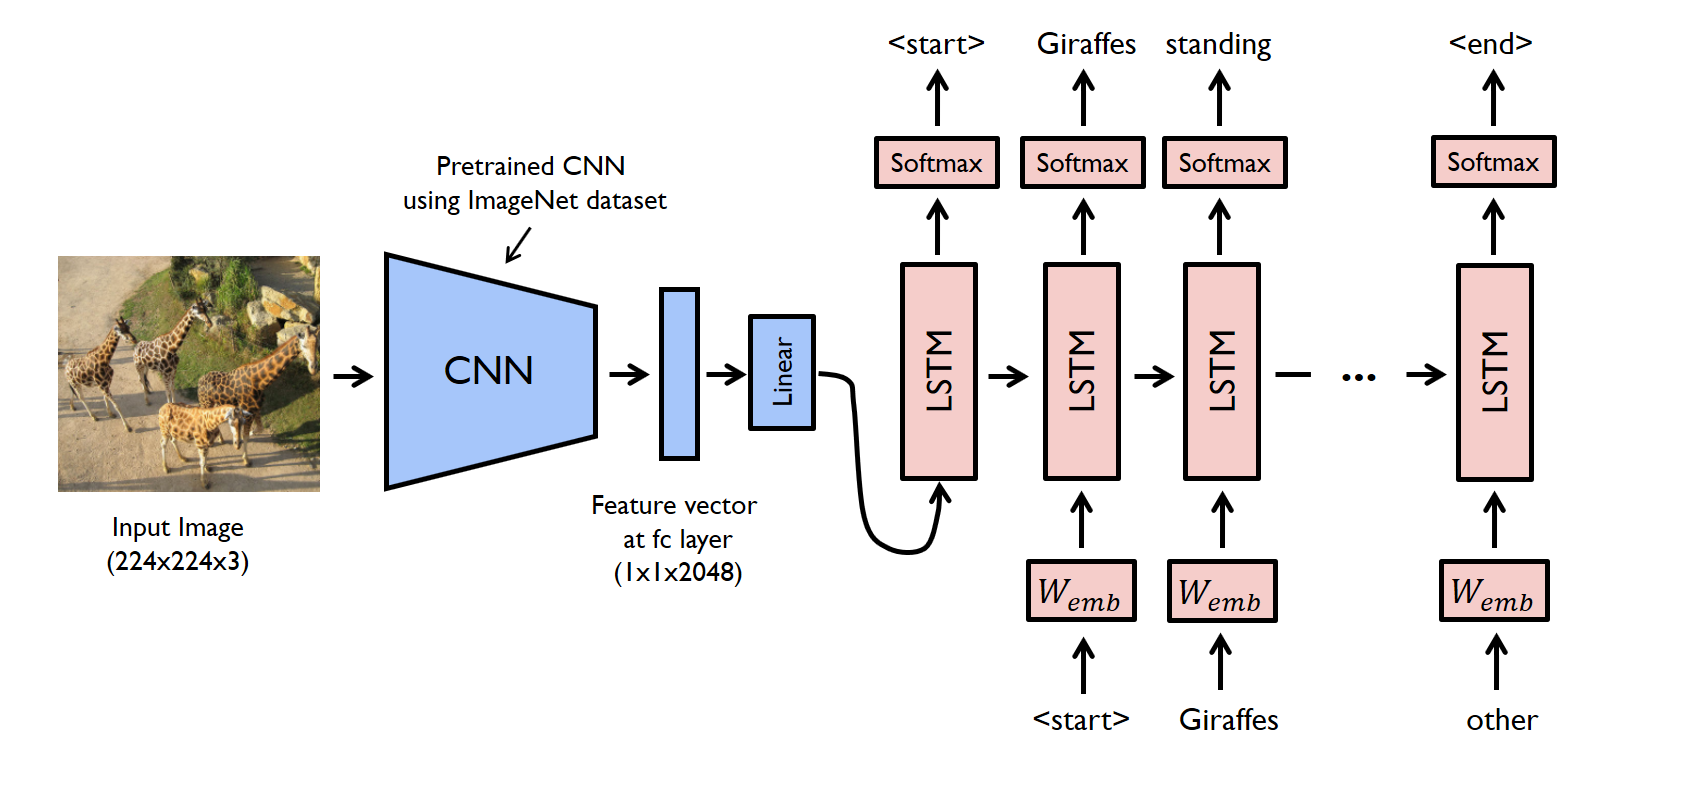
\includegraphics[scale=0.3]{images/ch3/cnn-rnn.png}
	\caption{Encoder-decoder combining CNN and LSTM for image captionign. Source:  \href{https://github.com/yunjey/pytorch-tutorial/tree/master/tutorials/03-advanced/image_captioning}{Yunjey Choi's implementation} of the Show and Tell model \citep{Vinyals2015}.}
	\label{fig:cnn-rnn}
\end{figure}

A key of this architecture is the use of a CNN that is pre-trained on a challenging image classification task, which is re-purposed as a feature extractor for the caption generating problem (this is called \textit{transfer learning}). Typically, a CNN trained on the ImageNet dataset is used for this purpose.

For the decoder, most systems proposed so far use LSTM units, since they are more powerful than other types of recurrent units, although lately, GRU units have also emerged as a viable alternative with similar capabilities bu reduced cost.

\subsection{Sequence to Sequence modelling}\label{subsec:seq2seq}

\subsubsection{Architecture of seq2seq model}

The sequence to sequence (seq2seq) model is based on the encoder-decoder architecture to generate a sequence output for a sequence input. Both the encoder and the decoder use recurrent neural networks to handle sequence inputs. The hidden state of the encoder is used directly to initialize the decoder hidden state to pass information from the encoder to the decoder.

\begin{figure}[hpt]
	\centering
	\includesvg{images/ch3/seq2seq.svg}
	\caption{The sequence to sequence model architecture.}
	\label{fig:seq2seq}
\end{figure}

The layers in the encoder and the decoder are illustrated in the following figure.

\begin{figure}[hpt]
	\centering
	\includesvg{images/ch3/seq2seq-details.svg}
	\caption{Layers in seq2seq model.}
	\label{fig:seq2seq_details}
\end{figure}

\subsubsubsection{The seq2seq encoder}

In the encoder, we use the word embedding layer to obtain a feature index from the word index of the input language and then input it into a multi-level recurrent layer, typicall made of gated recurrent units such as LSTM or GRU. The input for the encoder is a batch of sequences, which is 2-D tensor with shape (batch size, sequence length). The output consists of both the outputs of the recurrent units and the hidden states (and memory cells of the last time step if using LSTM).

The output shape returned by the encoder after performing forward calculation on the input is (number of time steps, batch size, number of hidden units). The shape of the multi-layer hidden state of the gated recurrent unit in the final time step is (number of hidden layers, batch size, number of hidden units). If GRU is used used the \textit{state}  contains only one element, which is the hidden state. If LSTM is used, the \textit{state} list will also contain another element, which is the memory cell.

\subsubsubsection{The seq2seq decoder}

We directly use the hidden state of the encoder in the final time step as the initial hidden state of the decoder. This requires that the encoder and decoder RNNs have the same numbers of layers and hidden units.

The forward calculation of the decoder is similar to the encoder's. The only difference is the addition of a dense layer with the hidden size to be the vocabulary size to output the predicted confidence score for each word.

\subsubsection{Training}

For each time step, the decoder outputs a vocabulary size confident score vector to predict words. Similar to language modeling, we can apply \textit{softmax} to obtain the probabilities and then use cross entropy loss to calculate the loss. 

But note that we padded the target sentences to make them have the same length. We would not like to compute the loss on the padding symbols. To solve that, a masked version of the loss function is used.

During training, if the target sequence has length $n$, we feed the first $n-1$ tokens into the decoder as inputs, and the last $n-1$ tokens are used as ground truth label. This is called \textit{Teacher Forcing}, and is depicted in \cref{fig:seq2seq}.

\subsubsection{Prediction}

In \cref{subsec:seq2seq}  we discussed how to train an encoder-decoder with input and output sequences that are both of variable length. In this section, we are going to introduce how to use the encoder-decoder to predict sequences of variable length.

\begin{figure}[hpt]
	\centering
	\includesvg{images/ch3/seq2seq_predict.svg}
	\caption{Sequence to sequence model predicting with greedy search.}
	\label{fig:seq2seq_predict}
\end{figure}

In general, prediction is done by feeding the same "<bos>" token to the decoder as training at time step 0. But the input token for a later time step is the predicted token from the previous time step, instead of the ground truth token used during training, as shown in \cref{fig:seq2seq_predict}.

Various approaches exist to predict the next token. For example, in greedy search, the token with the highest score at each time step is chosen and used to predict the next token. However, there are more sophisticated approaches, introduce below. 

\paragraph{Notation}

As in the previous section, when preparing to train the data set, we normally attach a special symbol "<eos>" after each sentence to indicate the termination of the sequence. We will continue to use this mathematical symbol in the discussion below. For ease of discussion, we assume that the output of the decoder is a sequence of text. Let the size of output text dictionary $\mathcal{Y}$ (contains special symbol "<eos>") be $\left|\mathcal{Y}\right|$, and the maximum length of the output sequence be $T'$. There are a total $\mathcal{O}(\left|\mathcal{Y}\right|^{T'})$ types of possible output sequences. All the subsequences after the special symbol "<eos>" in these output sequences will be discarded.


\subsubsubsection{Greedy Search}

First, we will take a look at a simple solution: greedy search. For any time step $t'$ of the output sequence, we are going to search for the word with the highest conditional probability from $|\mathcal{Y}|$ numbers of words, with

$$y_{t'} = \operatorname*{argmax}_{y \in \mathcal{Y}} \mathbb{P}(y \mid y_1, \ldots, y_{t'-1}, \boldsymbol{c})$$

as the output.  Once the "<eos>" symbol is detected, or the output sequence has reached its maximum length $T'$, the output is completed.

As we mentioned in out discussion of the decoder, the conditional probability of generating an output sequence based on the input sequence is $\prod_{t'=1}^{T'} \mathbb{P}(y_{t'} \mid y_1, \ldots, y_{t'-1}, \boldsymbol{c})$. We will take the output sequence with the highest conditional probability as the optimal sequence. The main problem with greedy search is that there is no guarantee that the optimal sequence will be obtained.

Take a look at the example in \cref{fig:s2s_prob1}. We assume that there are four words "A", "B", "C", and "<eos>" in the output dictionary.  The four numbers under each time step represent the conditional probabilities of generating "A", "B", "C", and "<eos>" at that time step.  At each time step, greedy search selects the word with the highest conditional probability. Therefore, the output sequence "A", "B", "C", "<eos>" will be generated in \cref{fig:s2s_prob1}. The conditional probability of this output sequence is $0.5\times0.4\times0.4\times0.6 = 0.048$.


\begin{figure}[hpt]
	\centering
	\includesvg{images/ch3/s2s_prob1.svg}
	\caption{The four numbers under each time step represent the conditional probabilities of generating "A", "B", "C", and "<eos>" at that time step. At each time step, greedy search selects the word with the highest conditional probability.}
	\label{fig:s2s_prob1}
\end{figure}

% TODO many error in references to figures in the next paragraph

Now, we will look at another example shown in \cref{fig:s2s_prob2}. Unlike in \cref{fig:s2s_prob1}, \cref{fig:s2s_prob2} selects the word "C" for it has the second highest conditional probability at time step 2. Since the output subsequences of time steps 1 and 2, on which time step 3 is based, are changed from "A" and "B" in \cref{fig:s2s_prob1} to "A" and "C" in \cref{fig:s2s_prob2}, the conditional probability of each word generated at time step 3 has also changed in \cref{fig:s2s_prob2}. We choose the word "B", which has the highest conditional probability. Now, the output subsequences of time step 4 based on the first three time steps are "A", "C", and "B", which are different from "A", "B", and "C" in \cref{fig:s2s_prob1}. Therefore, the conditional probability of generating each word in time step 4 in \cref{fig:s2s_prob2} is also different from that in \cref{fig:s2s_prob1}. We find that the conditional probability of the output sequence "A", "C", "B", "<eos>" at the current time step is $0.5\times0.3 \times0.6\times0.6=0.054$, which is higher than the conditional probability of the output sequence obtained by greedy search. Therefore, the output sequence "A", "B", "C", "<eos>" obtained by the greedy search is not an optimal sequence.

\begin{figure}[hpt]
	\centering
	\includesvg{images/ch3/s2s_prob2.svg}
	\caption{The four numbers under each time step represent the conditional probabilities of generating "A", "B", "C", and "<eos>" at that time step.  At time step 2, the word "C", which has the second highest conditional probability, is selected.}
	\label{fig:s2s_prob2}
\end{figure}

\subsubsubsection{Exhaustive Search}

If the goal is to obtain the optimal sequence, we may consider using exhaustive search: an exhaustive examination of all possible output sequences, which outputs the sequence with the highest conditional probability.

Although we can use an exhaustive search to obtain the optimal sequence, its computational overhead $\mathcal{O}(\left|\mathcal{Y}\right|^{T'})$ is likely to be excessively high. For example, when $|\mathcal{Y}|=10000$ and $T'=10$, we will need to evaluate $10000^{10} = 10^{40}$ sequences. This is next to impossible to complete. The computational overhead of greedy search is $\mathcal{O}(\left|\mathcal{Y}\right|T')$, which is usually significantly less than the computational overhead of an exhaustive search. For example, when $|\mathcal{Y}|=10000$ and $T'=10$, we only need to evaluate $10000\times10=1\times10^5$ sequences.

\subsubsubsection{Beam Search}

Beam search is an improved algorithm based on greedy search. It has a hyper-parameter named beam size. We set it to $k$. At time step 1, we select $k$ words with the highest conditional probability to be the first words of the $k$ candidate output sequences. For each subsequent time step, we are going to select the $k$ output sequences with the highest conditional probability from the total of $k\left|\mathcal{Y}\right|$ possible output sequences based on the $k$ candidate output sequences from the previous time step. These will be the candidate output sequence for that time step. Finally, we will filter out the sequences containing the special symbol "<eos>" from the candidate output sequences of each time step and discard all the subsequences after it to obtain a set of final candidate output sequences.

\begin{figure}[hpt]
	\centering
	\includesvg{images/ch3/beam_search.svg}
	\caption{The beam search process. The beam size is 2 and the maximum length of the output sequence is 3. The candidate output sequences are $A$, $C$, $AB$, $CE$, $ABD$, and $CED$. }
	\label{fig:beam_search}
\end{figure}

\cref{fig:beam_search} demonstrates the process of beam search with an example. Suppose that the vocabulary of the output sequence only contains five elements: $\mathcal{Y} = \{A, B, C, D, E\}$ where one of them is a special symbol “<eos>”. Set beam size to 2, the maximum length of the output sequence to 3. At time step 1 of the output sequence, suppose the words with the highest conditional probability $\mathbb{P}(y_1 \mid \boldsymbol{c})$ are $A$ and $C$. At time step 2, we compute $\mathbb{P}(A, y_2 \mid \boldsymbol{c}) = \mathbb{P}(A \mid \boldsymbol{c})\mathbb{P}(y_2 \mid A, \boldsymbol{c})$ and $\mathbb{P}(C, y_2 \mid \boldsymbol{c}) = \mathbb{P}(C \mid \boldsymbol{c})\mathbb{P}(y_2 \mid C, \boldsymbol{c})$ for all $y_2 \in \mathcal{Y}$, and pick the largest two among these 10 values: say $\mathbb{P}(A, B \mid \boldsymbol{c})$ and $\mathbb{P}(C, E \mid \boldsymbol{c})$. Then at time step 3, we compute $\mathbb{P}(A, B, y_3 \mid \boldsymbol{c}) = \mathbb{P}(A, B \mid \boldsymbol{c})\mathbb{P}(y_3 \mid A, B, \boldsymbol{c})$ and $\mathbb{P}(C, E, y_3 \mid \boldsymbol{c}) = \mathbb{P}(C, E \mid \boldsymbol{c})\mathbb{P}(y_3 \mid C, E, \boldsymbol{c})$ for all $y_3 \in \mathcal{Y}$, and pick the largest two among these 10 values: say $\mathbb{P}(A, B, D \mid \boldsymbol{c})$ and $\mathbb{P}(C, E, D \mid  \boldsymbol{c})$. As a result, we obtain 6 candidates output sequences: (1) $A$; (2)$C$; (3) $A$, $B$; (4)$C$, $E$; (5)$A$, $B$, $D$; and (6)$C$, $E$, $D$. In the end, we will get the set of final candidate output sequences based on these 6 sequences.

In the set of final candidate output sequences, we will take the sequence with the highest score as the output sequence from those below:

$$ \frac{1}{L^\alpha} \log \mathbb{P}(y_1, \ldots, y_{L}) = \frac{1}{L^\alpha} \sum_{t'=1}^L \log \mathbb{P}(y_{t'} \mid y_1, \ldots, y_{t'-1}, \boldsymbol{c}),$$

Here, $L$ is the length of the final candidate sequence and the selection for $\alpha$ is generally 0.75. The $L^\alpha$ on the denominator is a penalty on the logarithmic addition scores for the longer sequences above. The computational overhead $\mathcal{O}(k\left|\mathcal{Y}\right|T')$ of the beam search can be obtained through analysis. The result is a computational overhead between those of greedy search and exhaustive search. In addition, greedy search can be treated as a beam search with a beam size of 1. Beam search strikes a balance between computational overhead and search quality using a flexible beam size of $k$.

\subsection{Attention Mechanism}\label{sec:attention}

In \cref{subsec:seq2seq}, we encode the source sequence input information in the recurrent unit state, and then pass it to the decoder to generate the target sequence. A token in the target sequence may closely relate to some tokens in the source sequence instead of the whole source sequence. For example, when translating "Hello world." to "Bonjour le monde.", "Bonjour" maps to "Hello" and "monde" maps to "world". In the seq2seq model, the decoder may implicitly select the corresponding information from the state passed by the decoder. The attention mechanism, however, makes this selection explicit.

Attention is a generalized pooling method with bias alignment over inputs. The core component in the attention mechanism is the \textbf{attention layer}. An input of the attention layer is called a \textbf{query}. For a query, the attention layer returns the output based on its \textbf{memory}, which is a set of key-value pairs. To be more specific, assume a query $\mathbf{q}\in\mathbb R^{d_q}$, and the memory contains $n$ key-value pairs, $(\mathbf{k}_1, \mathbf{v}_1), \ldots, (\mathbf{k}_n, \mathbf{v}_n)$, with $\mathbf{k}_i\in\mathbb R^{d_k}$, $\mathbf{v}_i\in\mathbb R^{d_v}$. The attention layer then returns an output $\mathbf o\in\mathbb R^{d_v}$ with the same shape, such that each key has a value.

\begin{figure}[hpt]
	\centering
	\includesvg{images/ch3/attention.svg}
	\caption{The attention layer returns an output based on the input query and its memory.}
	\label{fig:attention}
\end{figure}

To compute the output, we first assume there is a score function $\alpha$ which measures the similarity between the query and a key. Then we compute all $n$ scores $a_1, \ldots, a_n$ by

$$a_i = \alpha(\mathbf q, \mathbf k_i).$$

Next we use \textit{softmax} to obtain the attention weights

$$b_1, \ldots, b_n = \textrm{softmax}(a_1, \ldots, a_n).$$

The output is then a weight sum of the values

$$\mathbf o = \sum_{i=1}^n b_i \mathbf v_i.$$

Different choices of the score function lead to different attention layers. We will discuss two commonly used attention layers in the rest of this section. 
% Before diving into the implementation, we first introduce a masked version of the softmax operator and explain a specialized $dot$ operator.

% \begin{itemize}
%     \item The masked softmax takes a 3-dim input and allows to filter out some elements by specifying valid lengths for the last dimension
%     \item The operator $dot$ takes two inputs $X$ and $Y$ with shapes $(b, n, m)$ and $(b, m, k)$, respectively. It computes $b$ dot products, with $Z[i,:,:]=dot(X[i,:,:], Y[i,:,:]$ for $i=1,\ldots,n$.   
% \end{itemize}

\subsubsection{Dot Product Attention}

The dot product assume the query has the same dimension than the keys, namely $\mathbf q, \mathbf k_i \in\mathbb R^d$ for all $i$. It computes the score by an inner product between the query and a key, and often then divided by $\sqrt{d}$ to make the scores less sensitive to the dimension $d$. In other words,

$$\alpha(\mathbf q, \mathbf k) = \langle \mathbf q, \mathbf k \rangle /\sqrt{d}.$$

Assume $\mathbf Q\in\mathbb R^{m\times d}$ contains $m$ queries and $\mathbf K\in\mathbb R^{n\times d}$ has all $n$ keys. We can compute all $mn$ scores by

$$\alpha(\mathbf Q, \mathbf K) = \mathbf Q \mathbf K^T /\sqrt{d}.$$

This attention mechanism could also include a dropout regularization mechanism (to randomly drop some attention weights).

\subsubsection{Multilayer Perception Attention}

In multilayer perception attention, we first project both query and keys into a common feature dimension.
% TODO unfinished sentence

To be more specific, assume learnable parameters $\mathbf W_k\in\mathbb R^{h\times d_k}$, $\mathbf W_q\in\mathbb R^{h\times d_q}$, and $\mathbf v\in\mathbb R^{p}$, then the score function is defined by

$$\alpha(\mathbf k, \mathbf q) = \mathbf v^T \text{tanh}(\mathbf W_k \mathbf k + \mathbf W_q\mathbf q). $$

It equals to concatenate the key and value in the feature dimension, and then feed into a single hidden-layer perception with hidden size $h$ and output size $1$. The hidden layer activation function is \textit{tanh}, and no bias is applied.

\subsubsection{Sequence to Sequence with Attention Mechanism}

In this section, we add the attention mechanism to the sequence to sequence model introduced in \cref{subsec:seq2seq} to explicitly select state. The following figure shows the model architecture for a decoding time step. As can be seen, the memory of the attention layer consists of the encoder outputs of each time step. During decoding, the decoder output from the previous time step is used as the query, the attention output is then fed into the decoder with the input to provide attentional context information.

\begin{figure}[hpt]
	\centering
	\includesvg{images/ch3/seq2seq_attention.svg}
	\caption{The second time step in decoding for the sequence to sequence model with attention mechanism.}
	\label{fig:seq2seq_attention}
\end{figure}

The layer structure in the encoder and the decoder is shown in the following figure.

\begin{figure}[hpt]
	\centering
	\includesvg{images/ch3/seq2seq-attention-details.svg}
	\caption{Layers in seq2seq model with attention.}
	\label{fig:seq2seq-attention-details}
\end{figure}

For the decoder of this model, we add a MLP attention layer which has the same hidden size as the LSTM layer. The state passed from the encoder to the decoder contains three items:

\begin{itemize}
    \item the encoder outputs of all time steps, which are used as the attention layer's memory with identical keys and values
    \item the hidden state of the last time step that is used to initialize the encoder's hidden state  
    \item valid lengths of the decoder inputs so the attention layer will not consider encoder outputs for padding tokens.
\end{itemize}

In each time step of decoding, we use the output of the last RNN layer as the query for the attention layer. Its output is then concatenated with the input embedding vector to feed into the RNN layer. Despite the RNN layer's hidden state also contains history information from decoder, the attention output explicitly selects the encoder outputs that are correlated to the query and suspends other non-correlated information.

The training loss is similar to the seq2seq model, because the sequences in the training dataset are relatively short. The additional attention layer doesn’t lead to a significant difference. But due to both attention layer computational overhead and we unroll the time steps in the decoder, this model is much slower than the seq2seq model without attention.